\documentclass{article}
\usepackage{amsmath}
\usepackage{amssymb}
\usepackage{graphicx}
\usepackage{bibentry}

\begin{filecontents}{references.bib}
@article{vae_arxiv_2014,
   author = {{Kingma}, D.~P and {Welling}, M.},
    title = "{Auto-Encoding Variational Bayes}",
  journal = {ArXiv e-prints},
archivePrefix = "arXiv",
   eprint = {1312.6114},
 primaryClass = "stat.ML",
 keywords = {Statistics - Machine Learning, Computer Science - Learning},
     year = 2013,
    month = dec,
   adsurl = {http://adsabs.harvard.edu/abs/2013arXiv1312.6114K},
  adsnote = {Provided by the SAO/NASA Astrophysics Data System}
}
@article{pylearn2_arxiv_2013,
    author = {Goodfellow, Ian J. and Warde-Farley, David and Lamblin, Pascal and Dumoulin, Vincent and Mirza, Mehdi and Pascanu, Razvan and Bergstra, James and Bastien, Fr{\'{e}}d{\'{e}}ric and Bengio, Yoshua},
     title = {Pylearn2: a machine learning research library},
   journal = {arXiv preprint arXiv:1308.4214},
      year = {2013},
       url = {http://arxiv.org/abs/1308.4214},
  abstract = {Pylearn2 is a machine learning research library. This does not just mean that it is a collection of machine learning algorithms that share a common API; it means that it has been designed for flexibility and extensibility in order to facilitate research projects that involve new or unusual use cases. In this paper we give a brief history of the library, an overview of its basic philosophy, a summary of the library's architecture, and a description of how the Pylearn2 community functions socially.}

@article{tsa,
   author = {{Cohen}, T. and {Welling}, M.},
    title = "{Learning the Irreducible Representations of Commutative Lie Groups}",
  journal = {ArXiv e-prints},
archivePrefix = "arXiv",
   eprint = {1402.4437},
 primaryClass = "cs.LG",
 keywords = {Computer Science - Learning},
     year = 2014,
    month = feb,
   adsurl = {http://adsabs.harvard.edu/abs/2014arXiv1402.4437C},
  adsnote = {Provided by the SAO/NASA Astrophysics Data System}

@incollection{sfa,
title = {Slow, Decorrelated Features for Pretraining Complex Cell-like Networks},
author = {Bengio, Yoshua and James S. Bergstra},
booktitle = {Advances in Neural Information Processing Systems 22},
editor = {Y. Bengio and D. Schuurmans and J.D. Lafferty and C.K.I. Williams and A. Culotta},
pages = {99--107},
year = {2009},
publisher = {Curran Associates, Inc.},
url = {http://papers.nips.cc/paper/3868-slow-decorrelated-features-for-pretraining-complex-cell-like-networks.pdf}
}
    }
\end{filecontents}

\begin{document}

\title{Visual SLAM using Variational Autoencoders}
\author{Kyle Kastner}

\maketitle
\subsection*{Introduction}
The goal of Simultaneous Localization and Mapping (SLAM) is to have a robot
which is able to be placed in an unknown environment and learn the obstacles
and potential paths available, while also learning where (in relation to these
obstacles) it is. Without systems that can be placed in new environments and
\emph{learn} to operate, many applications will remain off-limits to robotics.
SLAM is an active research area in the robotics community, with several key
components coming from research in statistics, computer vision, and
machine learning. The proposed approach falls into the category of
monocular (single-camera) visual (video sensors only) SLAM. 

\subsection*{Data Sources}
There are a wide variety of publicly available datasets for SLAM testing. 
This project will focus on visual SLAM using a single camera, so datasets with
recorded video of simple paths with varied landscape features will be ideal for
testing. The Computer Vision Group at Technische Universit\"at M\"unchen has a
wide variety of viable candidate datasets, featuring RGBD (red, green, blue, depth) camera feeds as well
as ground truth paths for comparison. There are several datasets which feature
small loops over variable features, usually tables, chairs, or textured walls.
\paragraph{}
The 'freiburg3\_nostructure\_texture\_near\_withloop\_validation' dataset 
features 1845 frames of 648x480 RGB data. This dataset has been wrapped with a
pylearn2 \cite{pylearn2_arxiv_2013} compatible dataset class, and functions
 with other pylearn2 code. We eventually plan to gather custom testing videos 
using a small quadrotor in a
controlled environment to test different strengths and weaknesses of the
variational autoencoder \cite{vae_arxiv_2014} (VAE) method versus standard 
algorithms used in visual SLAM.

\subsection*{Preprocessing}
The representation of the input data is very important. The most basic
preprocessing steps for the data are to reduce the dimensionality of each
frame, as well as reducing the number of frames per second. For the simplest
implementation, an additional transformation of RGB to greyscale was performed.
The current results were obtained by feeding each frame individually to a
VAE, but we expect that images will need to be shown as pairs to learn
relations.

\subsection*{Mathematics of the Variational Autoencoder}
The goal of the variational autoencoder is to maximize the lower bound on the
log likelihood of the data. Mathematically, this means optimizing the following
formula:

\begin{equation} \label{eq1}
    \text{log}\;\emph{p}_\theta(\bf{x}^{(1)}, \ldots, \bf{x}^{(N)}) = \sum^{N}_{i=1} \text{log}\; \emph{p}_\theta(\bf{x}^{(i)})\\
\end{equation}
\begin{equation} \label{eq2}
    \text{log}\; \emph{p}_\theta(\bf{x}^{(i)}) = D_{KL}(\emph{q}_\theta(\bf{z|x^{(i)}})\;||\;\emph{p}_\theta(\bf{z|x^{(i)}})) + \mathcal{L}(\theta, \phi; x^{(i)})\\
\end{equation}

Because the KL divergence is non-negative, the second term on the right hand
side is called the variational lower bound. It can be written as follows:

\begin{equation} \label{eq3}
    \text{log}\; \emph{p}_\theta(\bf{x}^{(i)}) \geq \mathcal{L}(\theta, \phi; x^{(i)})\\ = \mathbb{E}_{\emph{q}_{\phi}(\bf{z|x})}[-\text{log}\;\emph{q}_\phi(\bf{z|x}) + \text{log}\;\emph{p}_\theta(\bf{x, z})]
\end{equation}

\begin{equation} \label{eq4}
    \mathcal{L}(\theta, \phi; x^{(i)})\\ = -D_{KL}(\emph{q}_\phi(\bf{z|x^{(i)}})\;||\;\emph{p}_\theta(\bf{z})) + \mathbb{E}_{\emph{q}_\phi(\bf{z|x^{(i)}})}[\text{log}\;\emph{p}_\theta(\bf{x^{(i)}|z})]
\end{equation}

 By optimizing $\mathcal{L}$, we improve the variational lower bound on our
 data. This should mean that whether the lower bound itself is increasing, or
 the gap between the lower bound and the true log likelihood is decreasing.
 Both situations are favorable, though improving the true log likelihood
 is the ideal result.

\subsection*{Encoder and Decoder Techniques}
Three primary techniques are promising for good representation and decoding
of the input frames. Convolutional layers will take advantage of the structure
inherent in color images, and are currently being integrated into the VAE that
is already in pylearn2. However, it is unlikely that adding convolutional layers
will be effective for capturing the \emph{relationships} between images, 
which is critical since that is ultimately what is necessary for understanding
location within an environment. There may also be difficulties integrating
"deconvolution" into the decoder, though it may not be necessary to do 
deconvolution to reconstruct the input.
\paragraph{}
Another technique called Slow Feature
Analysis (SFA) \cite{sfa} is a better candidate for learning relationships, and has a body
of publication supporting its use for learning relationships between inputs, as
well as previous publications from the LISA lab performing this task using
neural networks %[Bergstra Bengio paper]. 
The third option is a new method known as Toroidal Subspace Analysis \cite{tsa}(TSA). It
is similar in many ways to SFA, but appears to be a more general approach to 
finding relationships between sets of features. At a high level TSA learns a
feature space rotation, which should in theory allow it to learn the kinds of
transformations we need to encode location, and is very similar to the
"slow changes" learned by SFA. This work seems quite promising, but as the TSA
technique is quite new, there may be more effort required to
implement a usable model, as well as additional overhead in analyzing results.
In return, this technique may be the most promising for our data and goals.
\paragraph{}
It may be feasible to mix and match these layers, but doing so will
require more engineering effort to ensure that all of the project code is
reliable. Mixing may also bring the problems of each technique
without the benefits, if the strengths of each type are canceled out by
subsequent layers during encoding and decoding.

\subsection*{Basic Results}
The current training plot was obtained using a simple feedforward multilayer perceptron (MLP) for both
encoding and decoding. A diagonal Gaussian prior, Bernoulli conditional, and
diagonal Gaussian prior were set as initial parameters. The preprocessing
parameters gave a grayscale input of size 28x28 (length 784 as a vector), with
a total of 1845 samples. These images were then fed separately into the VAE.
Hyperparameter search will be crucial, along with finding the
proper input representation, as the current setup does not appear to be
learning anything useful.

\begin{figure}[h!]
    \centering
    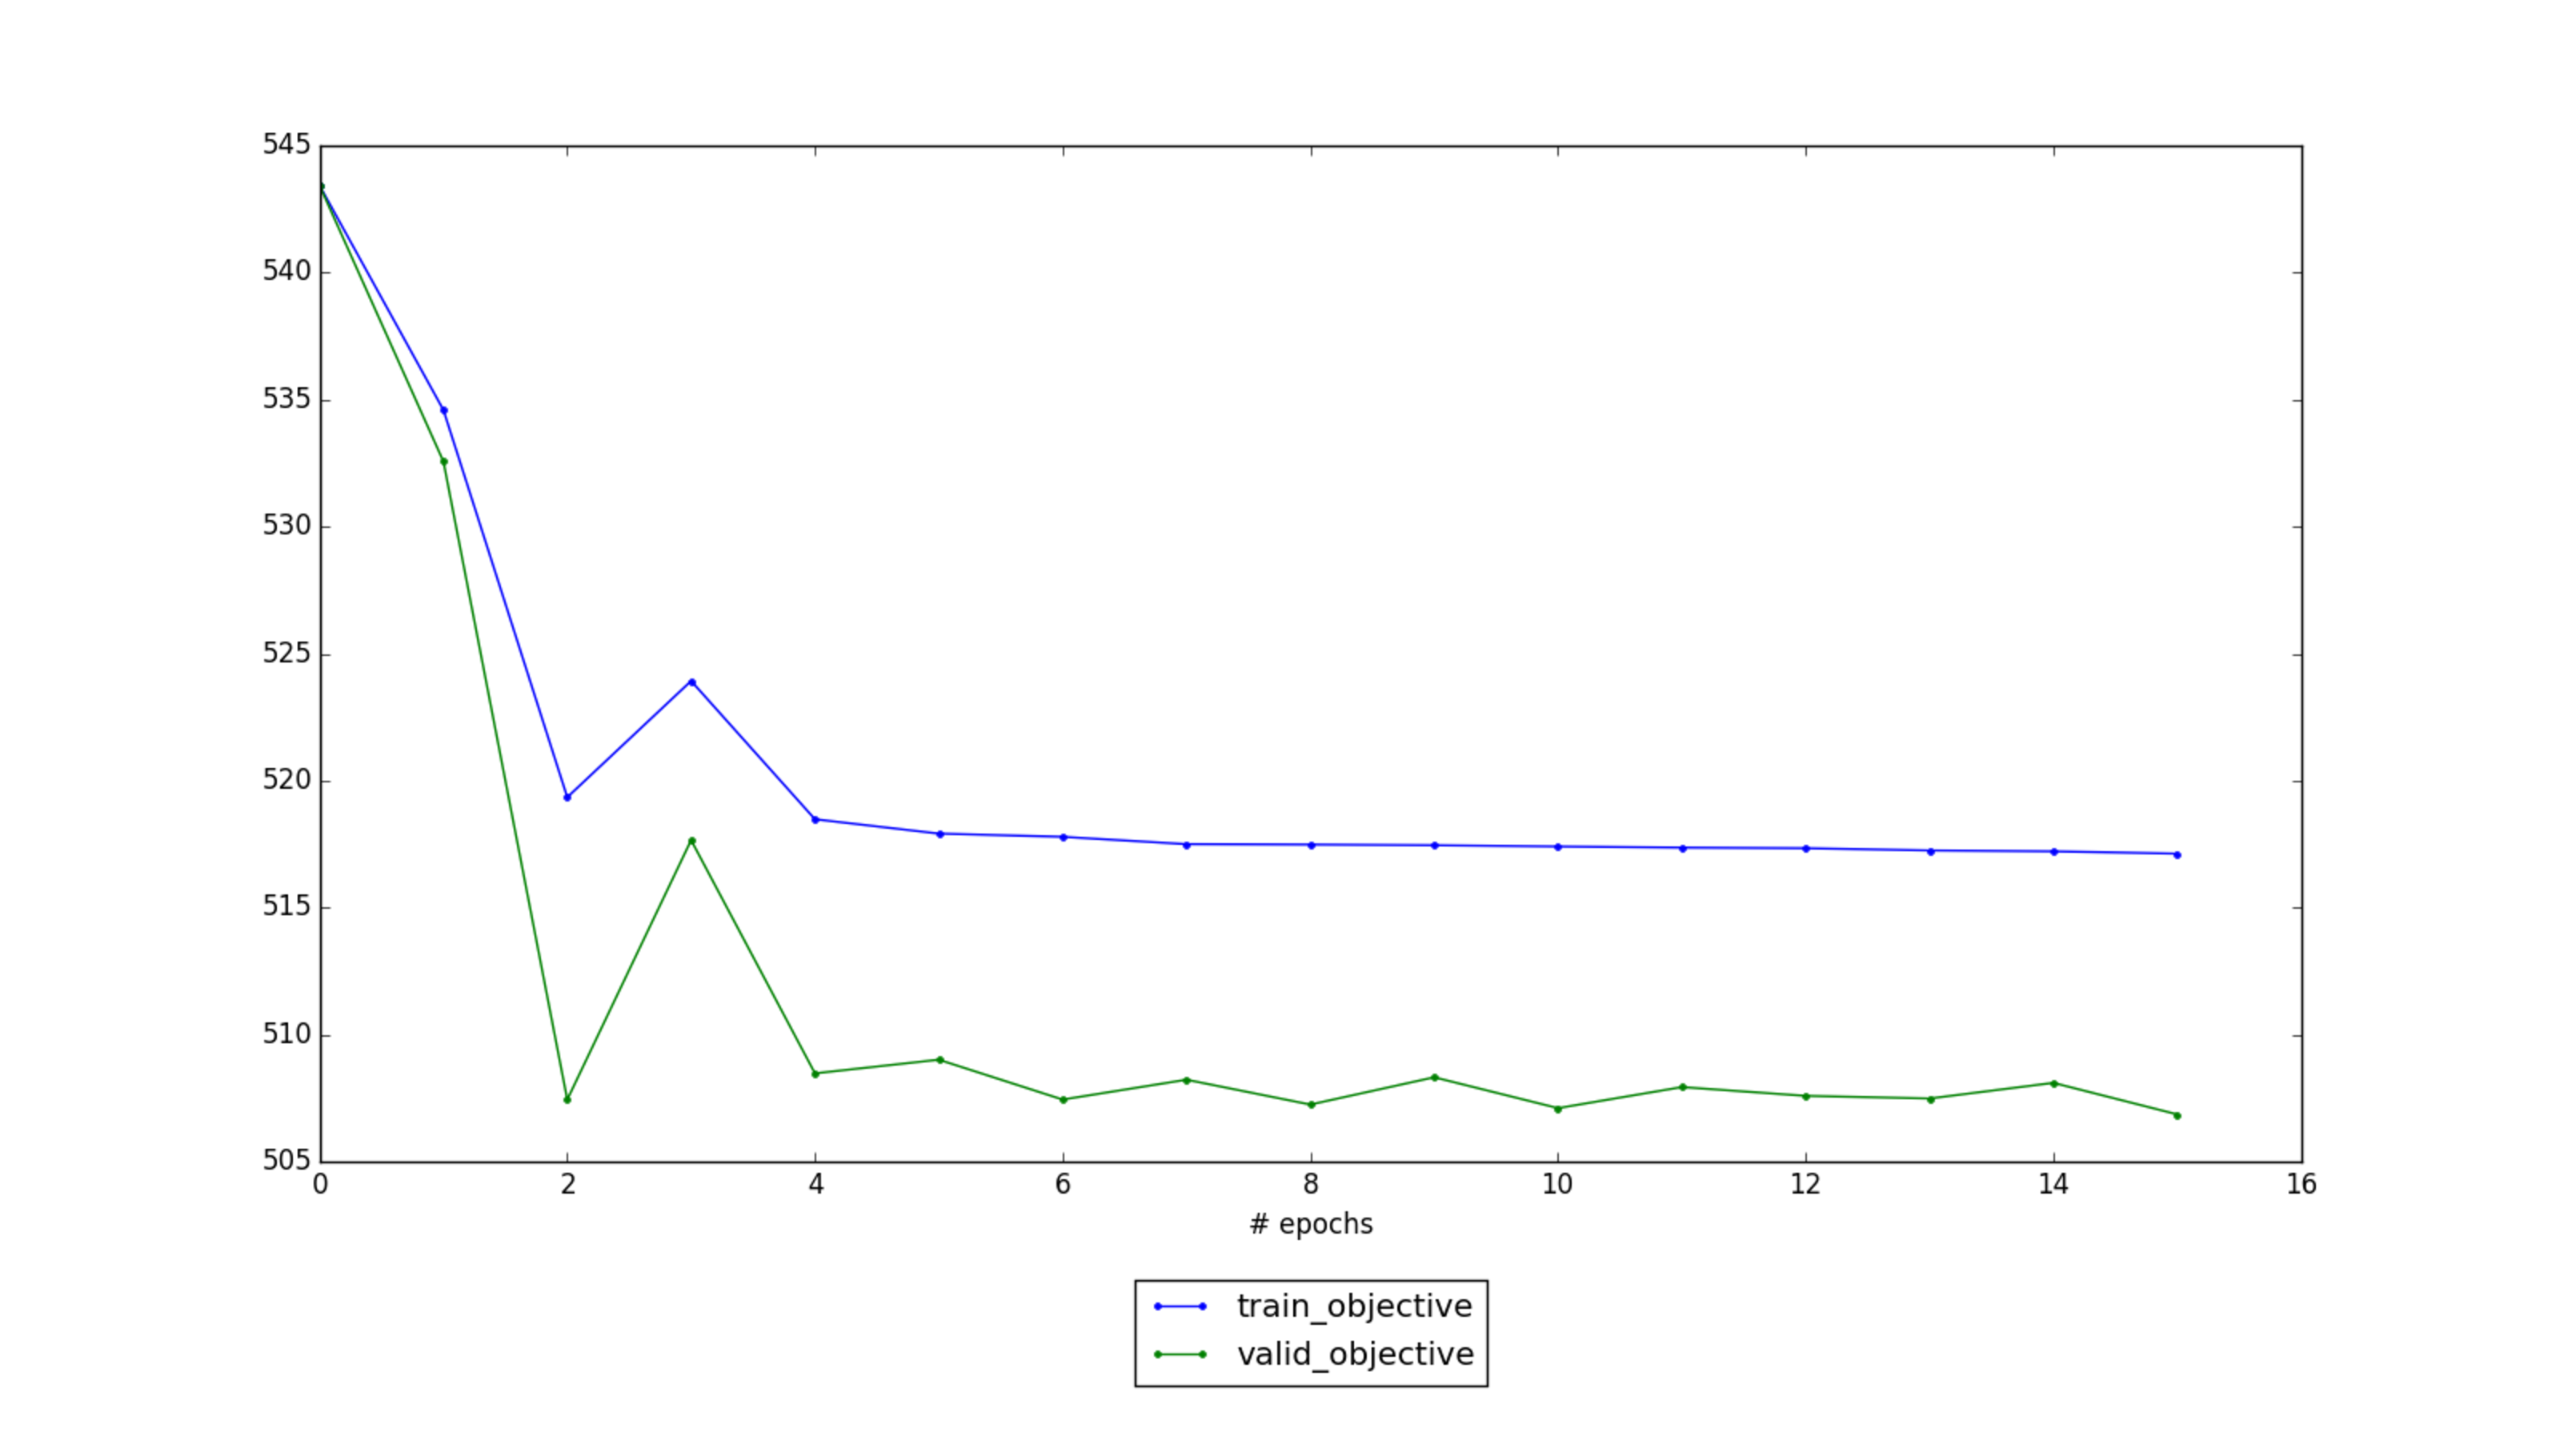
\includegraphics[width=0.8\textwidth,height=0.6\textwidth]{vae_basic_enlarged.png}
    \caption{Training and validation log likelihood for initial experiment}
\end{figure}


\subsection*{Completed Work}
\begin{itemize}
    \item Implement basic variational autoencoder on faces or audio
    \item Implement dataset class for example SLAM dataset in pylearn2
    \item Try basic variational autoencoder for example SLAM data 
    \item Find reference implementation of minimal visual SLAM algorithm
\end{itemize}

\subsection*{Items To Complete}
\begin{itemize}
    \item Get results of minimal SLAM pipeline for example dataset
    \item Extend into basic visual SLAM pipeline
    \item Integrate variational autoencoder into pipeline
    \item Explore different encoder/decoder hyperparameters
    \item Compare the two visual SLAM techniques (basic, VAE) on several datasets.
\end{itemize}

%\begin{itemize}
%    \item http://www.robots.ox.ac.uk/ActiveVision/Research/Projects/2003ajdi_monoslam/project.html
%    \item http://www.cc.gatech.edu/~dellaert/FrankDellaert/Frank_Dellaert/Entries/2014/6/28_Visual_SLAM_Tutorial_at_CVPR.html
%    \item https://openslam.org/ekfmonoslam.html
%    \item http://www.cvc.uab.es/adas/projects/slam/?page_id=14
%    \item http://ieeexplore.ieee.org/xpl/articleDetails.jsp?arnumber=6630554
%    \item http://ocw.mit.edu/courses/aeronautics-and-astronautics/16-412j-cognitive-robotics-spring-2005/projects/1aslam_blas_repo.pdf
%\end{itemize}
\bibliographystyle{plain}
\bibliography{references.bib}
\end{document}
